\chapter{Badania eksperymentalne}
\section{Organizacja eksperymentów}
W poniższym rozdziale wybrane modele z rozdziału \ref{chap:ChangeDetectionAlgo} zostaną,
w celu zbadania efektywności algorytmów,
przetestowane na losowych zbiorach danych.
Sekcja ta została podzielona na dwie części.
Pierwsza przedstawia szczegółową analizę problemu z wykorzystaniem badanych metod,
natomiast w części drugiej znajdują się zbiorcze wyniki przeprowadzonych doświadczeń.

Analizie eksperymentalnej zostaną poddane algorytmy:
\begin{itemize}
  \item Bayesa,
  \item ADWIN z testem opartym o średnią,
  \item ADWIN z testem opartym o stosunek gęstości rozkładu.
\end{itemize}

W badaniach będą wykorzystane zbiory danych wygenerowane losowo jak i rzeczywiste,
pochodzące z prawdziwych czujników.
\subsection*{Dane wygenerowane losowo}
\subsubsection*{Skacząca średnia}
Jednowymiarowy model auto-regresji wykorzystany przez Liu (Liu i in., 2013)
zostanie użyty do wygenerowania 5000 próbek.
Wartości są opisane wzorem:
$$y(t) = 0.6y(t-1) - 0.5y(t-2) + \varepsilon_t,$$
gdzie $\varepsilon_t$ jest szumem opisanych rozkładem Gaussa z średnią $\mu$
i odchyleniem standardowym równym 1,5.
Zmianie co 100 próbek ulegała średnia szumu $\mu$.
\[ \mu_N =
  \begin{cases}
    0       & \quad N = 1\\
    \mu_{N-1} + \frac{N}{16} & \quad N = 2,3, \ldots, \\
  \end{cases}
\]
gdzie N to liczba naturalna równa indeksowi aktualnej zmiany.
\subsubsection*{Rozkład dwuwymiarowy -- zmiana kowariancji}
Do badania użyto 5000 próbek pobranych z dwuwymiarowego rozkładu normalnego.
Zmiana występuje co 100 próbek
i polega na modyfikacji macierzy kowariancji $\Sigma$.
\[ \Sigma =
  \begin{cases}
    \begin{pmatrix} 1 & -\frac{4}{5} - \frac{N-2}{500} \\ -\frac{4}{5} - \frac{N-2}{500} & 1 \end{pmatrix} & \quad N = 1,3,\ldots\\
    \begin{pmatrix} 1 & \frac{4}{5} + \frac{N-2}{500} \\ \frac{4}{5} + \frac{N-2}{500} & 1 \end{pmatrix} & \quad N = 2,4,\ldots\\
  \end{cases}
\]

\subsection*{Dane rzeczywiste}
Dane rzeczywiste zebrano za pomocą czujnika światła oraz czujnika zbiżeniowego.
Czujniki leżały na biurku i skierowane pionowo w kierunku sufitu.
Przykładowe wyniki czujników przedstawiono w tabeli \ref{tab:DeviceValues}.
Wykres \ref{fig:DeviceValues} przedstawia przebiegi ostatnich 5000 próbek.
\subsubsection*{Czujnik światła}
Czujnik mierzył natężenie światła w otoczeniu.
Na wartości wpływ ma nie tylko fakt przesłonięcia go przez przedmiot,
ale także pora dnia.
\subsubsection*{Czujnik odległości}
Czujnik zbliżeniowy mierzy odległość od najbliższego przedmiotu,
wynik był podawany w cm.
\begin{table}[h]
  \label{tab:DeviceValues}
  \centering
  \begin{tabular}{r r}
    \multicolumn{1}{l}{Odległość} & \multicolumn{1}{l}{Natężenie} \\
    \hline
    266.34 & 0566 \\
    266.34 & 0567 \\
    266.32 & 0566 \\
    266.77 & 0566 \\
    266.84 & 0567 \\
    266.36 & 0567 \\
    266.73 & 0568 \\
    266.29 & 0566 \\
    266.68 & 0565 \\
    266.29 & 0566 \\
    266.36 & 0566 \\
    266.32 & 0567 \\
    266.72 & 0568 \\
    266.77 & 0567 \\
  \end{tabular}
  \caption{Wartości czujników}
\end{table}
\begin{figure}[htbp]
  \centering
  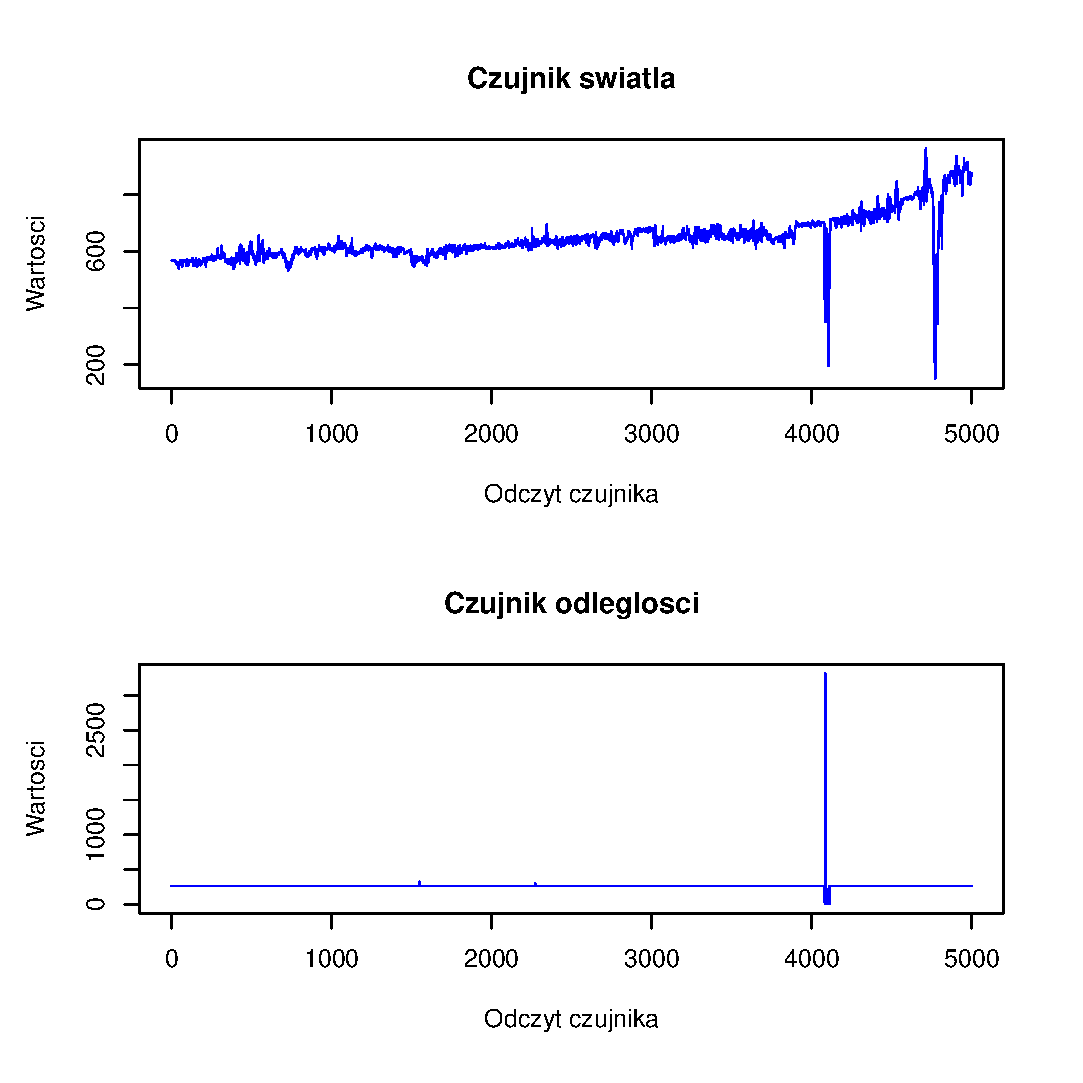
\includegraphics[width=1\textwidth]{img/ch-5-device}
  \caption{Wartości czujników}
  \label{fig:DeviceValues}
\end{figure}
\newpage
\section{Wyniki eksperymentów}
W poniższym rozdziale zostaną przedstawione wyniki przeprowadzonych badań.
\subsection{Studium przypadku}
\subsubsection*{Czujnik światła}

\subsection{Analiza modeli}
\subsection{Analiza porównawcza}
